\documentclass[twoside,10pt]{article}
\usepackage{shlists}
\usepackage[latin1]{inputenc}
\usepackage[spanish]{babel}
\usepackage[T1]{fontenc}


\usepackage{multicol}
\usepackage{picinpar}

\usepackage{url}
\newcommand{\surl}[1]{{\small\url{#1}}}

\newcounter{vol}
\newcounter{num}
\newcounter{anyo}
\setcounter{vol}{9}
\setcounter{num}{2}
\setcounter{anyo}{2016}
\newcommand{\mes}{Mayo}
\usepackage{revisionNLcol}


\title{\ \\ Docencia 2.0\\ \large Juan Juli\'{a}n Merelo, Fernando Tricas}
\author{\LARGE Dise\~nando un proyecto: {\em design thinking} para los estudios de inform\'atica}

\date{}

\AutTit{Docencia 2.0}

\begin{document}
\addtocounter{page}{2}

\maketitle
\vspace*{-5ex}

\begin{multicols}{2}

Uno de los problemas a los que se enfrentan tanto estudiantes como el profesorado
cuando tratan de proponer nuevos proyectos para una asignatura o TFG (de los
que hablamos, por cierto, no hace tanto en la columna `En defensa de los
trabajos de fin de grado'\footnote{ReVisi�n, Vol 9, No 2
(2016)~\url{http://www.aenui.net/ojs/index.php?journal=revision&page=article&op=view&path[]=238&path[]=381}}), 
es encontrar un tema que sea atractivo para el estudiante, que est\'e dentro
de la �rbita de los conocimientos de los dos, y que tambi\'en
lo acerque, dentro de lo posible, al mundo real, o al menos a un \'emulo del
mundo real suficientemente razonable. 

El cumplimiento de ese conjunto de restricciones hace que el campo
disponible se reduzca mucho: extensiones de proyectos anteriores,
proyectos en los que el estudiante est\'e en ese momento trabajando si es que est\'a
relacionado con una empresa, o peque\~nos proyectos relacionados con la
investigaci�n del tutor, suelen ser las soluciones m\'as socorridas. Sin embargo,
no siempre se pueden cumplir todas las restricciones y en ocasiones el
requisito que se suele caer de ese panel es el de acercarse al mundo real. O 
acercarse demasiado a una parte muy limitada de ese mundo que se reduce a los
intereses de quien realiza el proyecto, o de quien lo encarga.  Lo que es una
pena, porque como ya dijimos en la columna anterior sobre TFGs, proyectos
realizados, siempre que se liberen (o al menos se abran en un
repositorio), acaban formando parte de un portafolio que
ser\'a la carta de presentaci�n del estudiante ya graduado al mundo de la
empresa. Y el hecho de que el proyecto sea atractivo, bien
pensado, con un p\'ublico objetivo definido y no solo t\'ecnicamente correcto, puede aumentar su
empleabilidad considerablemente. Y tambi\'en la diversi�n: m\'as interaccci�n, m\'as variables que considerar y m\'as oportunidades.
El problema es que un proyecto poco atractivo y sin un p\'ublico objetivo
definido es dif\'icil que sea t\'ecnicamente correcto, por lo que una fase de
elecci�n y dise\~no adecuada es esencial para el \'exito del mismo.

La creaci�n del proyecto, en s\'i, es una t\'ecnica y tambi\'en una metodolog\'ia, y
una que se puede tambi\'en {\em aprobar} o {\em suspender}. Y que se
debe, y hay que aprender. Un proyecto llevado a
su t\'ermino pero cuyo p\'ublico objetivo est\'e mal pensado o no exista puede dar al
traste con el esfuerzo realizado. Y para ello est\'a la metodolog\'ia denominada,
por alguna raz�n en ingl\'es, {\em design thinking}, o {\em la forma en que
  piensan los dise\--\~nadores}, una metodolog\'ia que se ha impuesto
\'ultimamente en eventos de tipo {\em startup}, donde se trata de
dise\~nar una compa\~n\'ia alrededor de un producto dise\~nado de esta forma.
%Esta frase no termino de pillarla bien.
%Era una broma con el uso de t\'erminos ingleses. la quito. 
En todo caso, cuando hablamos de {\em design thinking} estamos
pensando en resoluci�n de tareas que requieran la aparici�n de un
enfoque creativo. Pero no hablamos de creatividad porque s\'i, sino una
creativididad dirigida a poner a las personas en el centro y sus necesidades como
objetivo. 

%--------------------------
\noindent\rule{86mm}{1pt}
\vspace{1ex} {\small{\begin{window}[0,r,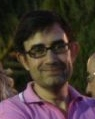
\includegraphics[width = 27mm]{JJM.jpg},] 
\noindent\emph{JJ Merelo} es catedr\'{a}tico de Universidad
en el \'area de Arquitectura y Tecnolog\'{\i}a de Computadores, y
actualmente director de la Oficina de Software Libre de la UGR.
Mantiene un blog desde el a\~no 2002, y lo ha utilizado en clase desde
el a\~no 2004; tambi\'en wikis, agregadores y repositorios de c\'odigo
como herramientas docente. \'{U}ltimamente le ha dado por el \textsl{flipped
learning}, de lo que se informar\'{a} debidamente en esta columna.
\end{window}}}

\medskip

{\small{\begin{window}[0,r,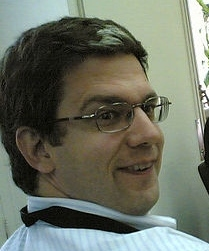
\includegraphics[width = 27 mm]{FTricas1.jpg},]
		\noindent \emph{Fernando Tricas Garc\'{\i}a} es profesor
		titular de Lenguajes y Sistemas Inform\'{a}ticos del Departamento
		de Inform\'{a}tica e Ingenier\'{\i}a de Sistemas de la Universidad de
		Zaragoza.  Empez\'{o} a estudiar la blogosfera casi cuando a\'{u}n no
		exist\'{\i}a (all\'{a} por el a\~{n}o 2002) y a tratar de integrarla en los
		cursos y tareas docentes un poco despu\'{e}s.  Ha impartido
		numerosas charlas relacionadas con el tema de la Web 2.0, 
		internet y universidad,\ldots\ 
		Es actualmente Vicerrector de Tecnolog\'{\i}as de la Informaci\'{o}n y
de la Comunicaci\'{o}n.   
		\end{window}}}
%-------------------------------------------------

Podemos ver propuestas para aplicar esta metodolog\'ia a los trabajos de fin de
grado por parte del Dr. Manuel Amezcua en la entrada del blog Gomeres, `C�mo
identificar una idea atractiva, original y relevante para el Trabajo de fin de
Grado (TFG)'~\footnote{http://index-f.com/gomeres/?p=1393} y en diferentes
presentaciones del mismo autor, aplicadas al grado de Enfermer\'ia; sin
embargo, no hemos encontrado ninguna referencia a su uso, en nuestro
idioma, y dirigido a la ense\~nanza universitaria de la inform\'atica. 

As\'i que habr\'a que empezar por ver c�mo podr\'iamos aplicarla en nuestro
caso. Aunque hay varias versiones,
de forma simplificada esta metodolog\'ia pasar\'ia por diferentes fases:

\begin{itemize}
\item {\bf Empat\'ia}. En esta fase se trata de identificar cu\'al es el
  objetivo de nuestro proyecto. El objetivo puede ser alguna empresa de
  nuestro entorno inmediato en la que se est\'en haciendo pr\'acticas (familia,
amigos, ...), una l\'inea de investigaci�n del departamento, el p\'ublico con un
perfil determinado, un grupo de edad o de localizaci�n espec\'ifica... Las
posibilidades son muchas. Tambi\'en podemos
buscar  estad\'isticas en la prensa, o elaborarlas por nuestra cuenta si
no existen, buscando, por ejemplo, qu\'e tipo de p\'ublico expresa qu\'e
necesidades o usa qu\'e tipo de aplicaciones. Aqu\'i es donde la
figura del tutor interviene: deber\'a buscar esas historias de problemas o nichos
de mercado donde una aplicaci�n inform\'atica podr\'ia traer una soluci�n. Y
siempre teniendo en cuenta que tras la identificaci�n del p\'ublico objetivo, hay
que {\em
    ponerse en su piel} y tratar de entender qu\'e necesitan y c�mo lo
  necesitan. En eso consiste empatizar.  
Pensemos que el p\'ublico objetivo, entre otras cosas, determina los casos de
uso, y estos a su vez el modo de interacci�n con el objeto del proyecto. Sin tener este
aspecto claro, se puede intentar crear un sistema de gesti�n de contenidos
universal que s�lo se pueda usar desde l\'inea de �rdenes o un juego para
personas mayores con poco contraste y que necesite reflejos r\'apidos,
dos errores grandes que proceden de no identificar, desde la primera
fase, el p\'ublico objetivo. 
\item {\bf Idear}: Es el siguiente paso en la labor de un
%Quito lo de primer paso porque entonces no se si tiene sentido la metodolog\'ia,
%pero c\'ambialo otra vez si no tengo raz�n.
%No, est\'a bien. Aunque yo quer\'ia decir que es una parte que s\'i suele
%usarse en ingenier\'ia. 
  ingeniero, aunque uno que s\'i nos resulta bastante m\'as
  familiar. Queremos proporcionar soluciones a ese p\'ublico objetivo, a
  esas 
historias de usuario que se habr\'an elaborado en la primera fase. Ideas que
fluyan libremente, sin pensar, en este punto, en c�mo llevarlas a cabo: s�lo
soluciones a problemas provenientes de esa identificaci�n (empat\'ia) con los
destinatarios del trabajo, teniendo en cuenta sus necesidades y sus capacidades.
\item {\bf Prototipar}: Eventualmente hay que quedarse con alguna de
  las ideas, teniendo en cuenta las restricciones t\'ecnicas o de otro
  tipo que tenga el proyecto. En  unos casos  se desechar\'an por poco pr\'acticas o simplemente
  demasiado extensas para el marco de nuestro proyecto. Y entramos en
territorio m\'as familiar de nuestro trabajo. A partir de ahora ya sabemos qu\'e
hacer, gracias a las herramientas t\'ecnicas y habilidades que hemos
desarrollado previamente para resolver problemas.   
\end{itemize}

En esta columna nos gusta hablar de innovaci�n en la ense\~nanza y
proponer nuevas pr\'acticas que mejoren la situaci�n actual. Y usar esta
metodolog\'ia en Inform\'atica ser\'ia innovador por partida doble: primero, porque
se tratar\'ia de una metodolog\'ia nueva en nuestra carrera, y segundo, porque este
tipo de metodolog\'ia realmente traer\'ia m\'as innovaci�n a este campo, el de los
proyectos, que se prestan a la exploraci�n y a andar por caminos poco
transitados. Tambi\'en porque las personas son las grandes olvidadas en muchos
proyectos (incluso comerciales y comercializados) lo que lleva a que,
a veces, los productos que tenemos que utilizar no cubren nuestras
necesidades. As\'i que pensemos como dise\~nadores en nuestros trabajos de
fin de grado. 



\noindent 
\bigskip

\noindent\emph{Todas las columnas de la serie Docencia 2.0
pueden descargarse en formato LaTeX desde
\surl{https://github.com/ReVision-Docencia-20/Columnas}}

\noindent\rule{90mm}{1pt}

{\small \noindent\copyright 2016 JJ. Merelo, F. Tricas. Este art\'{\i}culo es de acceso libre distribuido bajo los t\'{e}rminos
de la Licencia Creative Commons de Atribuci\'{o}n, que permite copiar,
distribuir y comunicar p\'{u}blicamente la obra en cualquier medio, s\'{o}lido
o electr\'{o}nico, siempre que se acrediten a los autores y fuentes
originales}

\end{multicols}
\end{document}
